\subsection{Schroedinger picture}
In the Schroedinger picture, we focus on the time evolution of qubit states:
\begin{equation}  
	|\psi\rangle = |\psi(t)\rangle 
\end{equation}

Measurements project these states onto eigenstates of the measurement operators via
a projection $P$, so:

\begin{equation}
    P_M^{\pm} |\psi\rangle = \frac{(M\pm \mathbb{I})|\psi\rangle}{2}
\end{equation}
Where $M$ is a matrix representation of the physical observable
 to be measured.
For example, a measurement of a single qubit's spin along the z-axis would be
represented as:
\begin{equation}
    M_Z = \left(
        \begin{array}{cc}
            1 & 0 \\
            0 & -1 \\
        \end{array}
        \right)
\end{equation}
And that measurement would perform a projection $P_Z$:
\begin{equation}
    P_Z^+ = \left(
        \begin{array}{cc}
            1 & 0 \\
            0 & 0 \\
        \end{array}
        \right)
    or
    P_Z^- = \left(
        \begin{array}{cc}
            0 & 0 \\
            0 & 1 \\
        \end{array}
        \right)
\end{equation}
on the state, depending on whether the measurement result yielded $+1$ or $-1$.

Therefore, to calculate the output of a quantum circuit in the Schroedinger
picture, simply apply the measurements and gates on the input states.
\begin{figure}[h!]
	\begin{center}
	\captionsetup{justification=centering,margin=2cm}
	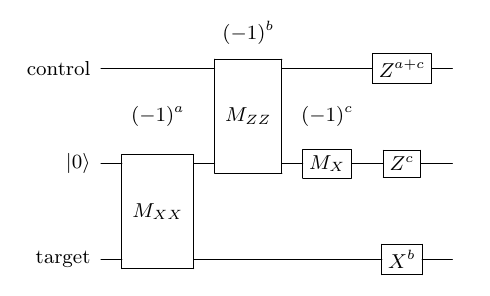
\includegraphics[scale=0.4]{img/figures/cnotMeasureCircuit.png}\\
	\caption{A Quantum Circuit to implement a measurement based\\
		Controlled-$X_{|\psi\rangle_{control}\rightarrow |\psi\rangle_{target}}$ Gate,
		where $|0\rangle$ is the +1 eigenstate in $\sigma_{z}$-basis.}
	\label{fig:circuit1}
	\end{center}
\end{figure}
As can be seen explicitly calculated in the Schroedinger 
picture in Appendix~\ref{sec:calc1}, the circuit from Figure~\ref{fig:circuit1}
implements a CNOT gate from the control qubit to the target qubit.

We will now analyze this circuit in the Heisenberg picture \cite{gottesman},
finding that it results in an equal output.

\subsection{Heisenberg picture and stabilizer formalism}
\subsubsection{Stabilizer group}
We call an operator/gate S, to which the input state is an
eigenvector ($S|\psi\rangle=|\psi\rangle$), a $stabilizer$ of that input state. 
For $n$-qubit systems, we write these stabilizers as $n$-tensor-products 
of pauli operators $P \in P_{G}$,
where $P_{G}$ is the group generated by the Pauli operators and
the Pauli operators are the operators on $\mathbb{F}_{2}$ such that:

\begin{equation}
    \forall P\in P_{G}: P^{2}=\mathbb{I}.
\end{equation}

In the Heisenberg picture, stabilizers are tracked instead of
states. 
The stabilizer group $S_{G}$ is the group generated by
the set of stabilizers:
\begin{equation}
	S_{G} = \langle S_{0},..,S_{n}\rangle: S|\psi_{in}\rangle = 
	|\psi_{in}\rangle \forall S \in S_{G}
\end{equation}

So for the example in Figure~\ref{fig:circuit1} it is the group
of operators to whom
$|\psi_{control}\rangle \otimes |0\rangle \otimes 
|\psi_{target}\rangle$ is an eigenstate, namely 
$\mathbb{I}\otimes Z \otimes \mathbb{I}$ (and trivially
$\mathbb{I}\otimes\mathbb{I}\otimes\mathbb{I}$, which we choose
to ignore as a stabilizer since any three-qubit state
is stabilized by it, and it can be generated by squaring any
stabilizer constructed through tensor products of Pauli matrices).

A stabilizer group is always an abelian group i.e. its elements 
 commute, since if:

\begin{equation}
	\label{abelian_stabilizers_equation}
	\forall A,B \in S: AB|\psi\rangle = BA|\psi\rangle = |\psi\rangle
	\Rightarrow [A,B]|\psi\rangle=0
\end{equation}

\subsubsection{Effect of gates on stabilizers}
To determine the effect a gate operation A has on a
stabilizer, consider the following:

If $S|\psi\rangle = |\psi\rangle$ then:
\begin{equation}
A|\psi\rangle = AS|\psi\rangle = AS\mathbb{I}|\psi\rangle
	= \underbrace{ASA^{\dagger}}_{=S'}A|\psi\rangle
\end{equation}
So we now know that the post-gate state is an eigenstate of $S'$.

Therefore $S'_{G} = \langle AS_{0}A^{\dagger},...,AS_{n}A^{\dagger}\rangle$.


\subsubsection{Effect of measurements on stabilizers}
After a measurement $M$, an $n$ qubit input state will always 
collapse into either the +1 or the -1 eigenstate of the 
measurement operator.
In the first case the acting measurement operator was 
$\mathbb{I}^{\otimes n}+M$, in the second it was
$\mathbb{I}^{\otimes n}-M$.

A Pauli measurement operator $M$ can either commute with all stabilizer
operators, in which case $M$ itself is a stabilizer already. In this case
the measurement has no effect on the state, since the measurement of a
stabilizer projects onto identity.
Otherwise it can anticommute with at
least one operator in $S_{G}$, since Pauli operators as well as
their tensor products can only commute or anti-commute with each
other. The product of two operators that both anticommute with another operator
will then commute with that operator.

So in order to obtain the new stabilizers  $S'_{G}$:
\begin{enumerate}
	\item Identify $S\in S_{G}: \{S,M\}=0$
	\item Remove S from $S_G$
	\item Add $M$ to $S_G$ 
	\item replace each $N \in S_G \cup\overline{X}\cup\overline{Z}$
		with SN if $\{N,M\}=0$
\end{enumerate}
where $\overline{X}$ and $\overline{Z}$ are the sets of 
logical X and Z operators respectively. A logical operator is
an operator which acts on a systems metastructure that can be treated
as its own qubit.

\subsubsection{Circuit Analysis in Stabilizer formalism}

In the following, stabilizers
will be written without the tensor product symbols, so in 
our case the stabilizer is initially: $S_{G}^{0}= \langle IZI \rangle$,
the logical $\overline{X}$ operator is XXX and the logical
$\overline{Z}$ operator is ZIZ.

 In the circuit shown in 
Figure~\ref{fig:circuit1}, the measurements project onto:

\begin{align}
	P^{\pm}_{1} &= \frac{1}{2}\left(\mathbb{I}^{\otimes 3} \pm 
	\mathbb{I}\otimes X \otimes X\right) \\
	P^{\pm}_{2} & = \frac{1}{2} \left(\mathbb{I}^{\otimes 3} \pm
	X \otimes X \otimes \mathbb{I}\right) \\
	P^{\pm}_{3} &= \frac{1}{2} \left(\mathbb{I}^{\otimes 3} \pm
	\mathbb{I} \otimes X \otimes \mathbb{I}\right)
\end{align}

After the first measurement, the state is stabilized by 
IXX, since it collapses into an eigenstate of the measurement 
operator. Notably, if the measurement operator M anticommutes
with some element of the stabilizer S:

\begin{equation}
	SP_{-}S^{\dagger} = \frac{1}{2}S\left( 
	\mathbb{I}^{\otimes 3} - M \right) S^{\dagger}
	= \frac{1}{2} \left( \mathbb{I}^{\otimes 3} + M \right)
	SS^{\dagger} = P_{+}
\end{equation}

So by applying an anticommuting previous stabilizer operator
after the measurement one can ensure that the state is in the
$P_{+}$ projected state $P_{+}|\psi_{init}\rangle$ (in short,
+1 and -1 eigenstates have the same stabilizers if we add 
conditional gates accordingly).

% For the logical operators, if $\overline{X}$ or $\overline{Z}$
% do not commute with the measurement operator, we know that their
% product with another anticommuting operator from the previous
% stabilizer must then commute with the measurement operator: 
% $[S_{prev}\overline{X}M, MS_{prev}\overline{X}]=0$ (recall the
% previous statement that all Paulis and their tensor products must
% either commute or anti-commute).

In our case, IZI and IXX anticommute,
so now the state is stabilized by $S^{1}_{G} = \langle IXX
\rangle$. Both initial logical operators commute with the first
measurement operator, so they are left unchanged.

After the second measurement $M_{2}$=ZZI, since this
measurement anticommutes with the IXX stabilizer, the new 
stabilizers are: $S^{2}_{G}=\langle ZZI \rangle$. The logical 
$\overline{X}$ and $\overline{Z}$ operators are unaffected
, since they commute with the measurement operator.

After the third measurement $M_{3}$ =IXI, since this measurement
anticommutes with the stabilizer, the new stabilizers are:
$S^{3}_{G}= \langle IXI \rangle$. The logical $\overline{Z}$
operator anticommutes with the measurement, so is replaced by\\
$ \overline{Z_{3}} $=ZZI $\cdot$ ZIZ = IIZ\@. The logical 
$ \overline{X} $ is unaffected since it commutes with the
measurement operator. 

The stabilizer for the control and target qubit is still
identity, and logical $\overline{Z}: ZIZ \rightarrow IIZ$.

Since this circuit maps $Z_{control}\otimes Z_{target} \mapsto I_{control}
 \otimes Z_{target}$,
and via a similar analysis it can be shown that it also maps
$I\otimes Z \mapsto Z \otimes Z$, $Z\otimes I \mapsto Z \otimes I$,
$X\otimes I \mapsto X \otimes X$ and $I\otimes X \mapsto I \otimes X$,
this circuit implements a logical CNOT from the first to the third qubit.
